% Options for packages loaded elsewhere
\PassOptionsToPackage{unicode}{hyperref}
\PassOptionsToPackage{hyphens}{url}
\documentclass[
  ignorenonframetext,
  aspectratio=169]{beamer}
\newif\ifbibliography
\usepackage{pgfpages}
\setbeamertemplate{caption}[numbered]
\setbeamertemplate{caption label separator}{: }
\setbeamercolor{caption name}{fg=normal text.fg}
\beamertemplatenavigationsymbolsempty
% remove section numbering
\setbeamertemplate{part page}{
  \centering
  \begin{beamercolorbox}[sep=16pt,center]{part title}
    \usebeamerfont{part title}\insertpart\par
  \end{beamercolorbox}
}
\setbeamertemplate{section page}{
  \centering
  \begin{beamercolorbox}[sep=12pt,center]{section title}
    \usebeamerfont{section title}\insertsection\par
  \end{beamercolorbox}
}
\setbeamertemplate{subsection page}{
  \centering
  \begin{beamercolorbox}[sep=8pt,center]{subsection title}
    \usebeamerfont{subsection title}\insertsubsection\par
  \end{beamercolorbox}
}
% Prevent slide breaks in the middle of a paragraph
\widowpenalties 1 10000
\raggedbottom
\AtBeginPart{
  \frame{\partpage}
}
\AtBeginSection{
  \ifbibliography
  \else
    \frame{\sectionpage}
  \fi
}
\AtBeginSubsection{
  \frame{\subsectionpage}
}
\usepackage{iftex}
\ifPDFTeX
  \usepackage[T1]{fontenc}
  \usepackage[utf8]{inputenc}
  \usepackage{textcomp} % provide euro and other symbols
\else % if luatex or xetex
  \usepackage{unicode-math} % this also loads fontspec
  \defaultfontfeatures{Scale=MatchLowercase}
  \defaultfontfeatures[\rmfamily]{Ligatures=TeX,Scale=1}
\fi
\usepackage{lmodern}
\ifPDFTeX\else
  % xetex/luatex font selection
\fi
% Use upquote if available, for straight quotes in verbatim environments
\IfFileExists{upquote.sty}{\usepackage{upquote}}{}
\IfFileExists{microtype.sty}{% use microtype if available
  \usepackage[]{microtype}
  \UseMicrotypeSet[protrusion]{basicmath} % disable protrusion for tt fonts
}{}
\makeatletter
\@ifundefined{KOMAClassName}{% if non-KOMA class
  \IfFileExists{parskip.sty}{%
    \usepackage{parskip}
  }{% else
    \setlength{\parindent}{0pt}
    \setlength{\parskip}{6pt plus 2pt minus 1pt}}
}{% if KOMA class
  \KOMAoptions{parskip=half}}
\makeatother
\setlength{\emergencystretch}{3em} % prevent overfull lines
\providecommand{\tightlist}{%
  \setlength{\itemsep}{0pt}\setlength{\parskip}{0pt}}
% ============================================================
% Custom Beamer Theme — IA-dem Presentation
% Minimalist, professional, teal/navy accent palette
% ============================================================

\usepackage{fontspec}
\usepackage{unicode-math}
\usepackage{booktabs}
\usepackage{colortbl}
\usepackage{amsmath}
\usepackage{tikz}
\usetikzlibrary{positioning, arrows.meta, calc}

% --- Color definitions ---
\definecolor{myNavy}{HTML}{1B2A4A}
\definecolor{myTeal}{HTML}{009988}
\definecolor{myRed}{HTML}{CC3311}
\definecolor{myAmber}{HTML}{EE7733}
\definecolor{myLight}{HTML}{F5F7FA}
\definecolor{myHighlight}{HTML}{FFF3E0}

% --- Beamer structure colors ---
\setbeamercolor{structure}{fg=myNavy}
\setbeamercolor{frametitle}{fg=myNavy, bg=white}
\setbeamercolor{subtitle}{fg=myTeal}
\setbeamercolor{author}{fg=myNavy}
\setbeamercolor{date}{fg=myNavy!60}
\setbeamercolor{normal text}{fg=myNavy!90}
\setbeamercolor{block title}{fg=white, bg=myTeal}
\setbeamercolor{block body}{bg=myLight}
\setbeamercolor{alerted text}{fg=myRed}
\setbeamercolor{example text}{fg=myTeal}
\setbeamercolor{item}{fg=myTeal}

% --- Section pages (colored background) ---
\AtBeginSection{%
  {%
  \setbeamercolor{background canvas}{bg=myNavy}%
  \begin{frame}[plain,c]
    \centering
    \textcolor{white}{\Large\bfseries\insertsection}
  \end{frame}
  }%
}

% --- Frame title with underline ---
\setbeamerfont{frametitle}{size=\large, series=\bfseries}
\setbeamertemplate{frametitle}{%
  \nointerlineskip
  \vspace{0.25cm}%
  \hbox to\hsize{\insertframetitle\hfil}%
  \vspace{-0.08cm}%
  \hbox to\hsize{{\color{myTeal}\leaders\hrule height 0.5pt\hfil}\hfil}%
  \vspace{0.05cm}%
}

% --- Title page ---
\setbeamerfont{title}{size=\Large, series=\bfseries}
\setbeamerfont{subtitle}{size=\normalsize}
\setbeamertemplate{title page}{%
  \vfill
  \begin{center}
    {\usebeamerfont{title}\textcolor{myNavy}{\inserttitle}}\\[8pt]
    {\usebeamerfont{subtitle}\textcolor{myTeal}{\insertsubtitle}}\\[16pt]
    {\usebeamerfont{author}\textcolor{myNavy}{\insertauthor}}\\[4pt]
    {\small\textcolor{myNavy!60}{\insertdate}}
  \end{center}
  \vfill
}

% --- No navigation, minimal footline ---
\setbeamertemplate{navigation symbols}{}
\setbeamertemplate{footline}{%
  \hfill%
  \raisebox{4pt}[0pt][0pt]{%
    \footnotesize\textcolor{myNavy!35}{\insertframenumber}%
  }%
  \hspace{10pt}\vspace{4pt}%
}

% --- Itemize styling ---
\setbeamertemplate{itemize item}{\textcolor{myTeal}{\small$\blacktriangleright$}}
\setbeamertemplate{itemize subitem}{\textcolor{myTeal!60}{\scriptsize$\triangleright$}}
\setbeamertemplate{enumerate items}[default]
\setbeamerfont{itemize/enumerate body}{size=\small}
\setbeamerfont{itemize/enumerate subbody}{size=\footnotesize}

% --- Tight spacing ---
\setlength{\parskip}{2pt}

% --- Shrink-to-fit for dense slides ---
\newcommand{\shrmark}{\vspace{0pt plus 1filll}}
\usepackage{booktabs}
\usepackage{longtable}
\usepackage{array}
\usepackage{multirow}
\usepackage{wrapfig}
\usepackage{float}
\usepackage{colortbl}
\usepackage{pdflscape}
\usepackage{tabu}
\usepackage{threeparttable}
\usepackage{threeparttablex}
\usepackage[normalem]{ulem}
\usepackage{makecell}
\usepackage{xcolor}
\usepackage{bookmark}
\IfFileExists{xurl.sty}{\usepackage{xurl}}{} % add URL line breaks if available
\urlstyle{same}
\hypersetup{
  pdftitle={AI Automation, Regime Type, and Crossed Fragility},
  pdfauthor={Manoel Galdino},
  hidelinks,
  pdfcreator={LaTeX via pandoc}}

\title{AI Automation, Regime Type, and Crossed Fragility}
\subtitle{From Sketch to Global Games: Revising a Formal Model}
\author{Manoel Galdino}
\date{April 2026}

\begin{document}
\frame{\titlepage}

\section{Motivation}\label{motivation}

\begin{frame}{The Question}
\protect\phantomsection\label{the-question}
\begin{center}
\Large How does AI automation affect regime stability?
\end{center}

\vspace{0.6cm}

\begin{columns}[T]
\begin{column}{0.48\textwidth}
\textbf{The economic premise}\\[4pt]
Automation can follow different \emph{trajectories} (Gans \& Goldfarb 2026):
\begin{itemize}
  \item \textbf{Rapid}: immediate displacement
  \item \textbf{Threshold}: complement first, substitute later
\end{itemize}
\end{column}
\begin{column}{0.48\textwidth}
\textbf{The political gap}\\[4pt]
Regime stability literature treats shocks by \emph{magnitude}, not \emph{shape}.\\[6pt]
No model asks: \emph{which trajectory is more dangerous for which regime?}
\end{column}
\end{columns}
\end{frame}

\begin{frame}{The Core Idea}
\protect\phantomsection\label{the-core-idea}
\begin{center}
\Large The same AI technology can \textcolor{myTeal}{\textbf{stabilize}} one regime\\
while \textcolor{myRed}{\textbf{destabilizing}} the other.
\end{center}

\vspace{0.5cm}

\begin{columns}[T]
\begin{column}{0.48\textwidth}
\centering\textbf{Rapid displacement}\\[4pt]
\textcolor{myTeal}{Democracies compensate}\\
\textcolor{myRed}{Autocracies face organized revolt}
\end{column}
\begin{column}{0.48\textwidth}
\centering\textbf{Threshold automation}\\[4pt]
\textcolor{myRed}{Democracies see no crisis until too late}\\
\textcolor{myTeal}{Autocracies contain disoriented workers}
\end{column}
\end{columns}

\vspace{0.4cm}

\begin{center}
\small This is the \textbf{crossed fragility} pattern.
\end{center}
\end{frame}

\begin{frame}{Roadmap}
\protect\phantomsection\label{roadmap}
\begin{columns}[T]
\begin{column}{0.48\textwidth}
\textbf{Part I --- The Original Paper}
\begin{enumerate}
  \item Model setup and v1 overview
  \item What worked, what didn't
\end{enumerate}
\vspace{0.2cm}
\textbf{Part II --- The Revision}
\begin{enumerate}
  \setcounter{enumi}{2}
  \item Strategy and key solutions
  \item Before/after comparison
\end{enumerate}
\end{column}
\begin{column}{0.48\textwidth}
\textbf{Part III --- The Welfare State}
\begin{enumerate}
  \setcounter{enumi}{4}
  \item Can democracies protect themselves?
  \item Social insurance as institutional insurance
\end{enumerate}
\vspace{0.2cm}
\textbf{Part IV --- Verification \& Lessons}
\begin{enumerate}
  \setcounter{enumi}{6}
  \item Lean 4 formalization
  \item What we learned
\end{enumerate}
\end{column}
\end{columns}
\end{frame}

\section{Part I: The Original Paper}\label{part-i-the-original-paper}

\begin{frame}{The Setup: What the Model Is About}
\protect\phantomsection\label{the-setup-what-the-model-is-about}
\small

A polity has \textbf{exposed workers} (\(E\)) facing AI automation over
\textbf{two periods}. Regime is \textbf{democracy} (\(D\)) or
\textbf{autocracy} (\(A\)). Workers choose: accept status quo (\(M\)) or
protest (\(P\)).

\vspace{0.1cm}

\renewcommand{\arraystretch}{1.1}
\begin{center}
\footnotesize
\begin{tabular}{p{1.3cm} p{4.8cm} p{5cm}}
\toprule
\textbf{Symbol} & \textbf{Meaning} & \textbf{Intuition} \\
\midrule
$\omega_t$ & Latent severity of automation & How bad the disruption really is \\
$\ell_t$ & Displacement ($0$ or $L$) & Did workers lose jobs? \\
$\varphi_t$ & Democratic compensation & How much democracy offsets loss \\
$\kappa_0, \eta_r$ & Repressive capacity $\times$ effectiveness & How well autocracy contains dissent \\
$\sigma$ & Signal noise (by trajectory) & How predictable is the shock? \\
$\pi^*$ & Equilibrium protest participation & Can workers coordinate? \\
$\beta$ & Complementarity gain ($\geq 0$) & AI temporarily boosts income \\
$w_E$ & Exposed worker's baseline wage & Income before automation \\
$\theta, W, k$ & Success share, total output, transition cost & Gains and costs of regime change \\
$\Delta$ & $\theta W \!-\! k \!-\! w_E$ (net revolt payoff) & Negative $\to$ no revolt without AI \\
\bottomrule
\end{tabular}
\end{center}

\vspace{0.05cm}

\textbf{Core asymmetry}: Democracy stabilizes by making \(M\)
\emph{attractive} (compensation). Autocracy by making \(P\)
\emph{costly} (repression).
\end{frame}

\begin{frame}{v1: Model Architecture}
\protect\phantomsection\label{v1-model-architecture}
\begin{center}
\resizebox{0.92\textwidth}{!}{%
\begin{tikzpicture}[
  box/.style={draw=myNavy, thick, rounded corners=3pt,
              minimum width=2.4cm, minimum height=0.7cm,
              font=\footnotesize, text=myNavy, align=center},
  arr/.style={->, thick, myNavy!70}
]
\node[box] (traj) at (0,0) {Trajectory $j \in \{r, \tau\}$};
\node[box] (a3)   at (3.8,0.7)  {A3: compensation reactive};
\node[box] (a4)   at (3.8,-0.7) {A4: repression by shock};
\node[box] (stab) at (7.4,0)    {Stability conditions};
\node[box] (cross) at (10.8,0)  {Crossed fragility};

\draw[arr] (traj) -- (a3);
\draw[arr] (traj) -- (a4);
\draw[arr] (a3) -- (stab);
\draw[arr] (a4) -- (stab);
\draw[arr] (stab) -- (cross);
\end{tikzpicture}%
}
\end{center}

\vspace{0.3cm}

\begin{itemize}
  \item Two periods, two trajectories, two regimes
  \item Five behavioral/structural assumptions (A1--A5)
  \item Binary displacement: $\ell_t \in \{0, L\}$
  \item Short, direct proofs
\end{itemize}
\end{frame}

\begin{frame}{v1: The Assumptions}
\protect\phantomsection\label{v1-the-assumptions}
\renewcommand{\arraystretch}{1.25}
\begin{center}
\footnotesize
\begin{tabular}{p{0.8cm} p{4.5cm} p{5.8cm}}
\toprule
 & \textbf{Content} & \textbf{Plain language} \\
\midrule
A1 & $\Delta < 0$ & Without automation, no one revolts \\
A2 & $L > |\Delta|$ & The shock is big enough to trigger revolt \\
\rowcolor{myHighlight} A3 & $\varphi_t = \bar{\varphi}$ if displaced, else 0 & \textbf{Democracy only compensates during visible crises} \\
\rowcolor{myHighlight} A4 & $\eta_r < 1$, $\eta_\tau = 1$ & \textbf{Repression degrades under rapid, holds under threshold} \\
A5 & Capacity built in $t\!=\!1$ persists & Institutions are slow to build \\
\bottomrule
\end{tabular}
\end{center}

\vspace{0.2cm}

\begin{center}
\small A3 and A4 are the \textbf{load-bearing} assumptions --- and both are \emph{directly imposed}, not derived from any deeper mechanism.
\end{center}
\end{frame}

\begin{frame}{v1: Results at a Glance}
\protect\phantomsection\label{v1-results-at-a-glance}
\begin{table}[!h]
\centering\begingroup\fontsize{9}{11}\selectfont

\begin{tabular}[t]{lll}
\toprule
\textcolor[HTML]{1B2A4A}{\textbf{}} & \textcolor[HTML]{1B2A4A}{\textbf{Content}} & \textcolor[HTML]{1B2A4A}{\textbf{Role}}\\
\midrule
P1 & Democratic fragility pattern & Core\\
P2 & Autocratic fragility pattern & Core\\
\cellcolor[HTML]{E8F5F0}{\textbf{P3}} & \cellcolor[HTML]{E8F5F0}{\textbf{Crossed fragility}} & \cellcolor[HTML]{E8F5F0}{\textbf{Core}}\\
P4 & Welfare cost of autocratic stability & Core\\
P5--P6 & Threshold of thresholds, interval width & Secondary\\
P7--P8 & Welfare state as insurance & Secondary\\
P9 & Endogenous fiscal fragility & Extension\\
\bottomrule
\end{tabular}
\endgroup{}
\end{table}
\end{frame}

\begin{frame}{v1: What Worked}
\protect\phantomsection\label{v1-what-worked}
\begin{columns}[T]
\begin{column}{0.48\textwidth}
\textcolor{myTeal}{\textbf{Strengths}}
\begin{itemize}
  \item Clear, testable result (crossed fragility)
  \item Parsimonious --- 15 pages, clean proofs
  \item Good numerical example
  \item Welfare state extension is natural
  \item Five-type regime typology
\end{itemize}
\end{column}
\begin{column}{0.48\textwidth}
\textcolor{myAmber}{\textbf{The foundation was solid}}\\[6pt]
The \emph{intuition} was right: trajectory determines which regime is fragile.\\[6pt]
The \emph{formalization} needed work: too short a distance from assumptions to results.
\end{column}
\end{columns}
\end{frame}

\section{Part I-B: Problems}\label{part-i-b-problems}

\begin{frame}{Problem 1: Behavioral Assumptions Imposed}
\protect\phantomsection\label{problem-1-behavioral-assumptions-imposed}
\begin{center}
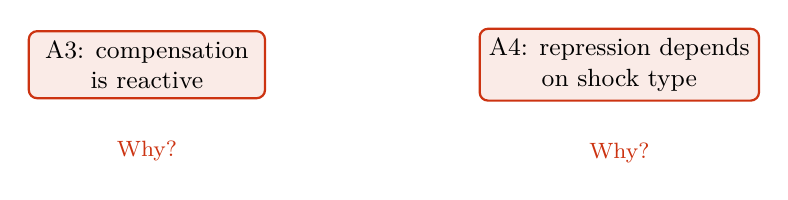
\begin{tikzpicture}[
  box/.style={draw=myRed, thick, rounded corners=3pt,
              minimum width=3cm, minimum height=0.7cm,
              font=\small, align=center},
  arr/.style={->, thick, myRed!70}
]
\node[box, fill=myRed!10] (a3) at (0,0) {A3: compensation\\is reactive};
\node[box, fill=myRed!10] (a4) at (6,0) {A4: repression depends\\on shock type};

\node[font=\footnotesize, text=myRed, below=0.4cm of a3] {Why?};
\node[font=\footnotesize, text=myRed, below=0.4cm of a4] {Why?};
\end{tikzpicture}
\end{center}

\vspace{0.4cm}

\begin{itemize}
  \item A3 \emph{assumes} democracies only compensate when job losses are visible --- but \emph{why} do democracies behave this way? No mechanism given.
  \item A4 \emph{assumes} repression works well against surprised workers but not organized ones --- but \emph{why}? Just postulated.
  \item Both describe exactly \textbf{the pattern we want to explain}, stated as premises
  \item A referee could say: ``the crossed fragility is \emph{assumed}, not proven''
\end{itemize}
\end{frame}

\begin{frame}{Problem 2: Binary Shock --- No Microfoundation}
\protect\phantomsection\label{problem-2-binary-shock-no-microfoundation}
\begin{columns}[T]
\begin{column}{0.55\textwidth}
In v1, the shock severity ($\omega$, ``how bad is automation?'') was binary --- workers are either displaced or not:
$$\ell_t \in \{0, L\}$$
\begin{itemize}
  \item No continuous \emph{signal space} for workers to form beliefs about others
  \item Global games (Morris \& Shin 2003) need continuous $\omega$ for unique equilibrium
  \item Appendix B \emph{sketched} coordination but main proofs didn't \emph{use} it
\end{itemize}
\end{column}
\begin{column}{0.42\textwidth}
\begin{center}
\textbf{The gap:}\\[6pt]
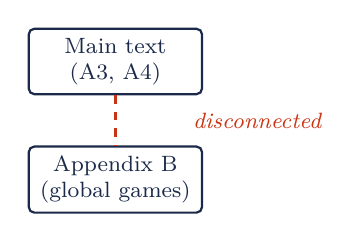
\begin{tikzpicture}[
  box/.style={draw=myNavy, thick, rounded corners=2pt,
              minimum width=2.2cm, minimum height=0.6cm,
              font=\footnotesize, text=myNavy, align=center}
]
\node[box] (main) at (0,1.5) {Main text\\(A3, A4)};
\node[box] (app)  at (0,0)   {Appendix B\\(global games)};
\node[font=\footnotesize\itshape, text=myRed] at (1.8,0.75) {disconnected};
\draw[dashed, myRed, thick] (main) -- (app);
\end{tikzpicture}
\end{center}
\end{column}
\end{columns}
\end{frame}

\begin{frame}{Problems 3--4: Short Distance and Sparse Presentation}
\protect\phantomsection\label{problems-34-short-distance-and-sparse-presentation}
\begin{columns}[T]
\begin{column}{0.52\textwidth}
\textbf{Short inferential distance}\\[4pt]
\resizebox{0.95\columnwidth}{!}{%

\begin{tikzpicture}[
  box/.style={draw=myNavy, thick, rounded corners=2pt,
              minimum width=2.2cm, minimum height=0.55cm,
              font=\footnotesize, text=myNavy, align=center},
  arr/.style={->, very thick, myRed!60}
]
\node[box] (prem)  at (0,0) {A3, A4};
\node[box] (conc)  at (4,0) {Crossed fragility};
\draw[arr] (prem) -- node[above, font=\scriptsize\itshape, text=myRed]
  {too direct} (conc);
\end{tikzpicture}%
}\\[4pt]
\small Results should \emph{emerge} from deeper primitives, not be \emph{restated} as assumptions.
\end{column}
\begin{column}{0.45\textwidth}
\textbf{Sparse presentation}\\[4pt]
\small v1 had:
\begin{itemize}
  \item No figures in main text
  \item No mechanism diagram
  \item No coordination plot
  \item No income path visualization
\end{itemize}
\vspace{0.1cm}
Reader must build mental model entirely unaided.
\end{column}
\end{columns}
\end{frame}

\section{Part II: The Revision}\label{part-ii-the-revision}

\begin{frame}{Revision Strategy}
\protect\phantomsection\label{revision-strategy}
\begin{center}
\large\textbf{One primitive, everything derived.}
\end{center}

\vspace{0.4cm}

\begin{columns}[T]
\begin{column}{0.48\textwidth}
\textbf{Goal:} Replace behavioral A3/A4 with a \emph{single informational primitive} ($\sigma$) from which both compensation and repression emerge as equilibrium outcomes.\\[6pt]
\textbf{Tool:} Global games (Morris \& Shin 2003) moved from appendix to core.
\end{column}
\begin{column}{0.48\textwidth}
\textbf{Changes:}
\begin{enumerate}
  \item Shock severity $\omega$: binary $\to$ continuous
  \item Compensation \& repression: assumed $\to$ derived from coordination equilibrium $\pi^*$
  \item Assumptions unbundled (5 $\to$ 7)
  \item Income paths: absorbing state + $\beta$ (AI temporarily boosts income before displacing)
  \item Four new figures
  \item Formal Lean 4 verification
\end{enumerate}
\end{column}
\end{columns}
\end{frame}

\begin{frame}{Solution 1: Continuous \(\omega\) + Global Games}
\protect\phantomsection\label{solution-1-continuous-omega-global-games}
\small\textit{How do we make compensation and repression \textbf{emerge} from a single mechanism?}

\vspace{0.1cm}

\begin{columns}[T]
\begin{column}{0.50\textwidth}
\textbf{New information structure}\\[3pt]
Each worker observes a \emph{private signal}:
$$s_{it} = \omega_t + \sigma_j \varepsilon_{it}$$
\vspace{-0.2cm}
\begin{itemize}
  \item $\omega_t$: true severity (now continuous)
  \item $\sigma_j$: noise, depends on trajectory
  \item $\varepsilon_{it}$: individual perception error
\end{itemize}

\vspace{0.1cm}
\footnotesize\textit{If $\omega\!=\!0.8$ and $\sigma$ is low (rapid), worker sees $s_i \!\approx\! 0.8$. If $\sigma$ is high (threshold), she might see $0.3$ or $1.5$ --- she can't tell how bad things are.}
\end{column}
\begin{column}{0.46\textwidth}
\textbf{Why this works}\\[3pt]
\begin{itemize}
  \item Continuous $\omega$ $\to$ Morris-Shin uniqueness theorem
  \item Uniform prior $\to$ Laplacian property $\to$ closed-form statics
  \item $\sigma$ is the \emph{single} trajectory-varying primitive
  \item Everything follows from $\pi^*(\sigma)$
\end{itemize}
\end{column}
\end{columns}
\end{frame}

\begin{frame}{Solution 1 (cont.): The Coordination Curve}
\protect\phantomsection\label{solution-1-cont.-the-coordination-curve}
\begin{center}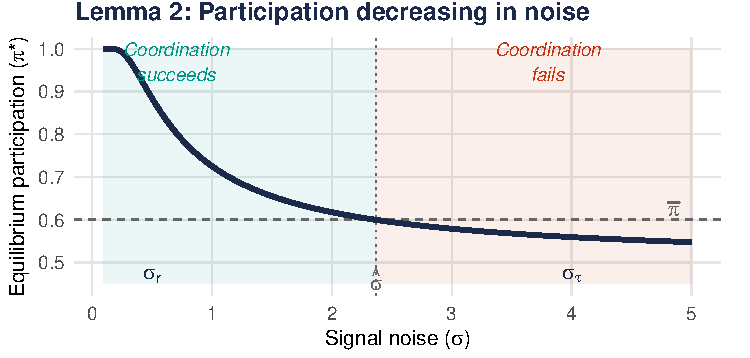
\includegraphics{presentation_files/figure-beamer/fig-threshold-1} \end{center}

\footnotesize \(\bar{\pi}\): minimum participation for collective action
to succeed. \(\hat{\sigma}\): critical noise at which coordination
breaks down. Curve plotted at \(\omega_0 = 1\) (realized shock severity
when displacement occurs).
\end{frame}

\begin{frame}{Solution 2: Assumptions Unbundled}
\protect\phantomsection\label{solution-2-assumptions-unbundled}
\renewcommand{\arraystretch}{1.2}
\begin{center}
\small
\begin{tabular}{p{0.7cm} p{3.5cm} p{0.4cm} p{0.7cm} p{4.8cm}}
\toprule
\multicolumn{2}{c}{\textbf{v1}} & & \multicolumn{2}{c}{\textbf{v2}} \\
\cmidrule(r){1-2} \cmidrule(l){4-5}
A3 & Compensation reactive & $\to$ & A3 & Information structure (M-S) \\
   &                        &      & A4 & Majority-cost condition \\
   &                        &      & A5 & Risk dominance \\
\addlinespace
A4 & $\eta_r$ by shock type  & $\to$ & A6 & Trajectory separation \\
\addlinespace
A5 & Capacity is a stock    & $\to$ & A7 & Institutional lead time \\
\bottomrule
\end{tabular}
\end{center}

\vspace{0.3cm}

\textbf{Key insight:} The old behavioral A3 \emph{bundled} three
distinct conditions --- the information structure, the voting game, and
the risk dominance selection. Unbundling makes each testable and
transparent.
\end{frame}

\begin{frame}{Solution 3: The New Architecture}
\protect\phantomsection\label{solution-3-the-new-architecture}
\begin{center}
\resizebox{0.95\textwidth}{!}{%
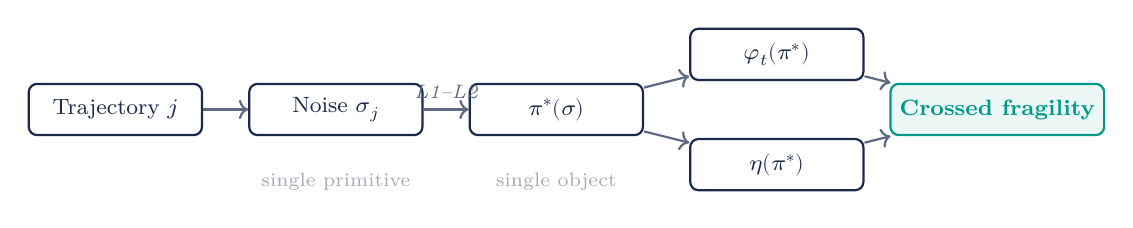
\begin{tikzpicture}[
  box/.style={draw=myNavy, thick, rounded corners=3pt,
              minimum width=2.2cm, minimum height=0.65cm,
              font=\footnotesize, text=myNavy, align=center},
  result/.style={draw=myTeal, thick, rounded corners=3pt,
                 minimum width=2.2cm, minimum height=0.65cm,
                 font=\footnotesize\bfseries, text=myTeal, align=center,
                 fill=myTeal!8},
  arr/.style={->, thick, myNavy!70}
]
\node[box] (traj) at (0,0) {Trajectory $j$};
\node[box] (sigma) at (2.8,0) {Noise $\sigma_j$};
\node[box] (pi) at (5.6,0) {$\pi^*(\sigma)$};
\node[box] (dem) at (8.4,0.7) {$\varphi_t(\pi^*)$};
\node[box] (aut) at (8.4,-0.7) {$\eta(\pi^*)$};
\node[result] (cross) at (11.2,0) {Crossed fragility};

\draw[arr] (traj) -- (sigma);
\draw[arr] (sigma) -- node[above, font=\scriptsize\itshape] {L1--L2} (pi);
\draw[arr] (pi) -- (dem);
\draw[arr] (pi) -- (aut);
\draw[arr] (dem) -- (cross);
\draw[arr] (aut) -- (cross);

\node[font=\scriptsize, text=myNavy!40, below=0.35cm of sigma] {single primitive};
\node[font=\scriptsize, text=myNavy!40, below=0.35cm of pi] {single object};
\end{tikzpicture}%
}
\end{center}

\vspace{0.3cm}

\begin{center}
The \textbf{inferential chain} is now: trajectory $\to$ $\sigma$ $\to$ $\pi^*$ $\to$ institutional map $\to$ stability.\\
\emph{One primitive, one equilibrium, two outcomes.}
\end{center}
\end{frame}

\begin{frame}{Solution 4: Income Paths Redesigned}
\protect\phantomsection\label{solution-4-income-paths-redesigned}
\begin{center}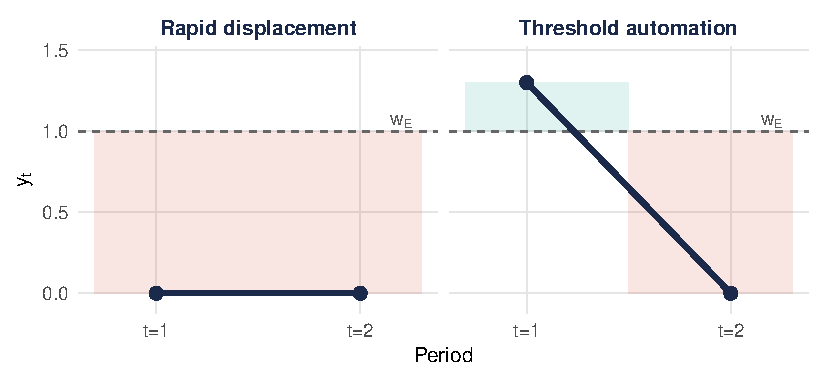
\includegraphics{presentation_files/figure-beamer/fig-income-paths-1} \end{center}

\footnotesize v1: \(\ell_1\!=\!L, \ell_2\!=\!0\)
vs.~\(\ell_1\!=\!0, \ell_2\!=\!L\). v2: rapid is an
\textbf{absorbing state} (loss persists); threshold has a
\textbf{complementarity gain} \(\beta\) (AI boosts income before
replacing workers).
\end{frame}

\begin{frame}{Solution 5: The Four Scenarios}
\protect\phantomsection\label{solution-5-the-four-scenarios}
\small\textit{Before I show you: which cell do you think is unstable? Democracy under rapid, or under threshold?}

\vspace{0.1cm}

\begin{center}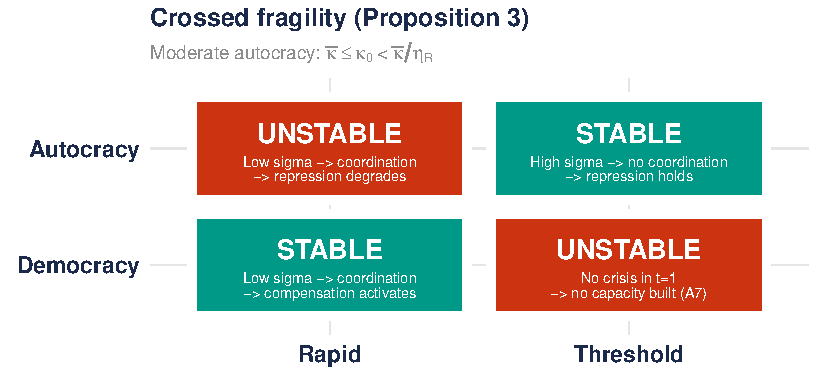
\includegraphics{presentation_files/figure-beamer/fig-four-scenarios-1} \end{center}
\end{frame}

\section{Part II-B: Before vs.~After}\label{part-ii-b-before-vs.-after}

\begin{frame}{Propositions: Before and After}
\protect\phantomsection\label{propositions-before-and-after}
\renewcommand{\arraystretch}{1.15}
\begin{center}
\small
\begin{tabular}{p{0.6cm} p{3.5cm} p{3.3cm} p{3.8cm}}
\toprule
 & \textbf{Content} & \textbf{v1} & \textbf{v2} \\
\midrule
P1 & Democratic fragility & Uses A3 directly & Uses L1--L2 + A7 \\
P2 & Autocratic fragility & Uses A4 directly & Uses L1--L2 \\
P3 & Crossed fragility & Combines A3+A4 & Single $\pi^*$ object \\
P4 & Welfare cost & Same & Same \\
\addlinespace
R1 & Threshold of thresholds & Was P5 & Now a Remark \\
R2 & Interval width & Was P6 & Now a Remark \\
\addlinespace
P5 & Welfare state insurance & Was P7 & Rewritten with $\varphi_0$ \\
P6 & Functional equivalence & Was P8 & Tighter proof \\
P7 & Fiscal fragility & Was P9 & Endogenous constraint \\
\bottomrule
\end{tabular}
\end{center}
\end{frame}

\begin{frame}{The Parametric Space}
\protect\phantomsection\label{the-parametric-space}
\begin{center}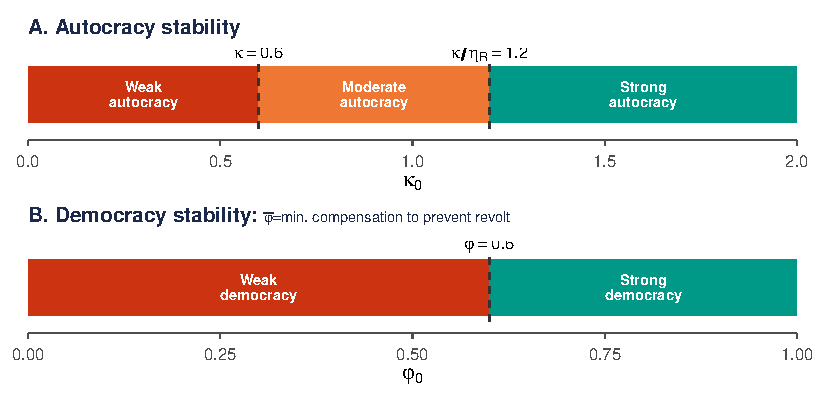
\includegraphics{presentation_files/figure-beamer/fig-parametric-1} \end{center}
\end{frame}

\begin{frame}{The Complete Typology}
\protect\phantomsection\label{the-complete-typology}
\begin{center}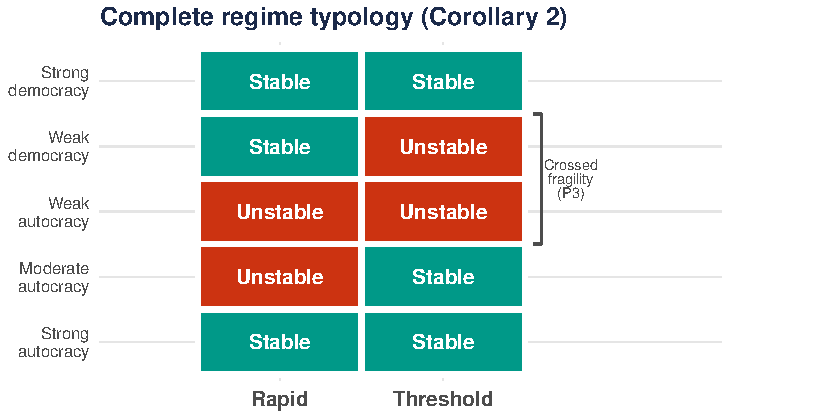
\includegraphics{presentation_files/figure-beamer/fig-typology-1} \end{center}
\end{frame}

\section{Part III: The Welfare State}\label{part-iii-the-welfare-state}

\begin{frame}{Can Democracies Protect Themselves?}
\protect\phantomsection\label{can-democracies-protect-themselves}
The new architecture reveals a natural question: if the coordination
bottleneck is what makes democracies fragile under threshold automation,
can they \textbf{bypass} it?

\vspace{0.3cm}

\begin{columns}[T]
\begin{column}{0.48\textwidth}
\textbf{The problem}\\[4pt]
Weak democracies need a visible crisis to trigger compensation. Threshold shocks provide no visible crisis until too late (A7).
\end{column}
\begin{column}{0.48\textwidth}
\textbf{The solution}\\[4pt]
Build \emph{standing} compensation ($\varphi_0$) \emph{before} the shock --- a welfare state that does not require crisis activation.\\[4pt]
$\varphi_0$ is the democratic analogue of $\kappa_0$ (standing repression).
\end{column}
\end{columns}
\end{frame}

\begin{frame}{Insurance Against Delayed Shocks}
\protect\phantomsection\label{insurance-against-delayed-shocks}
\begin{columns}[T]
\begin{column}{0.55\textwidth}
\textbf{P5:} Democracy stable under threshold iff standing compensation $\varphi_0 \geq \bar{\varphi}$ (the compensatory threshold --- how much compensation is needed to keep workers from revolting).\\[4pt]

The welfare state \textbf{bypasses the coordination bottleneck}: it works even when workers can't organize.\\[4pt]

\textbf{P6:} Both strong democracies and strong autocracies survive both trajectories. But the welfare gap is $\bar{\kappa} = L - |\Delta|$ (the repressive threshold):
\vspace{0.1cm}
\centerline{$u_E^D - u_E^A \geq \bar{\kappa} > 0$}
\end{column}
\begin{column}{0.42\textwidth}
\begin{center}
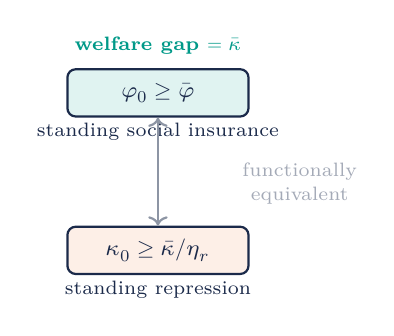
\begin{tikzpicture}[
  box/.style={draw=myNavy, thick, rounded corners=3pt,
              minimum width=2.3cm, minimum height=0.6cm,
              font=\footnotesize, text=myNavy, align=center}
]
\node[box, fill=myTeal!12] (dem) at (0,2) {$\varphi_0 \geq \bar{\varphi}$};
\node[font=\scriptsize, text=myNavy] at (0,1.5) {standing social insurance};
\node[box, fill=myAmber!12] (aut) at (0,0) {$\kappa_0 \geq \bar{\kappa}/\eta_r$};
\node[font=\scriptsize, text=myNavy] at (0,-0.5) {standing repression};
\node[font=\scriptsize, text=myNavy!40] at (1.8,1) {functionally};
\node[font=\scriptsize, text=myNavy!40] at (1.8,0.7) {equivalent};
\node[font=\scriptsize\bfseries, text=myTeal] at (0,2.6)
  {welfare gap $= \bar{\kappa}$};
\draw[<->, thick, myNavy!50] (dem.south) -- (aut.north);
\end{tikzpicture}
\end{center}
\end{column}
\end{columns}
\end{frame}

\begin{frame}{The Class Compromise Formalized}
\protect\phantomsection\label{the-class-compromise-formalized}
\begin{center}
\textbf{Social insurance protects both the regime and its citizens.}\\
\textbf{Repression protects only the regime.}
\end{center}

\vspace{0.2cm}

\begin{columns}[T]
\begin{column}{0.48\textwidth}
\small
\textbf{Numerical example:}\\[2pt]
Strong democracy ($\varphi_0 = 0.6$): $u_E = w_E - 0.4$\\[3pt]
Strong autocracy ($\kappa_0 = 0.8$): $u_E = w_E - 1.0$\\[3pt]
Gap: $0.6 = \bar{\kappa}$ \checkmark
\end{column}
\begin{column}{0.48\textwidth}
\small
\textbf{Przeworski \& Wallerstein (1982):}\\[2pt]
Workers consent to profit in exchange for protection.\\[3pt]
\textbf{Our formalization:} When institutionalized, this compromise insures the \emph{regime itself} against technological disruption.
\end{column}
\end{columns}
\end{frame}

\section{Part IV: Verification \&
Lessons}\label{part-iv-verification-lessons}

\begin{frame}{Lean 4 Formal Verification}
\protect\phantomsection\label{lean-4-formal-verification}
\begin{columns}[T]
\begin{column}{0.48\textwidth}
\small
\textbf{What we verified:}
\begin{itemize}
  \item P1--P7: all propositions
  \item R1--R2: remarks
  \item Coordination conditions
  \item Single-crossing, dominance regions
\end{itemize}
\vspace{0.1cm}
\textbf{17/17 verified.} Including L1--L2 (SupermodularGames lib).
\end{column}
\begin{column}{0.48\textwidth}
\small
\textbf{Why it matters:}
\begin{itemize}
  \item Every algebraic step machine-checked
  \item Caught two sign errors in drafts
  \item Forces precision in assumptions
  \item Builds reviewer confidence
\end{itemize}
\vspace{0.1cm}
\texttt{cd formal\_proofs \&\& lake build}
\end{column}
\end{columns}
\end{frame}

\begin{frame}{Comparative Statics Summary}
\protect\phantomsection\label{comparative-statics-summary}
\begin{table}[!h]
\centering\begingroup\fontsize{9}{11}\selectfont

\resizebox{\ifdim\width>\linewidth\linewidth\else\width\fi}{!}{
\begin{tabular}[t]{lll}
\toprule
\textcolor[HTML]{1B2A4A}{\textbf{Parameter}} & \textcolor[HTML]{1B2A4A}{\textbf{Effect}} & \textcolor[HTML]{1B2A4A}{\textbf{Interpretation}}\\
\midrule
$L \uparrow$ & $\bar{\varphi} \uparrow$, $\bar{\kappa} \uparrow$ & Larger shocks destabilize both\\
$\eta_r \downarrow$ & Crossed interval widens & More autocracies exhibit crossed pattern\\
$\theta \uparrow$ & $\Delta \uparrow$, thresholds rise & Regime change more attractive\\
$k \uparrow$ & $\Delta \downarrow$, thresholds fall & Regime change costlier\\
$\kappa_0 \uparrow$ & Autocracy more stable & Weak $\to$ moderate $\to$ strong\\
$\varphi_0 \uparrow$ & Democracy more stable (threshold) & Welfare state as insurance\\
\bottomrule
\end{tabular}}
\endgroup{}
\end{table}
\end{frame}

\begin{frame}{Lessons from the Revision}
\protect\phantomsection\label{lessons-from-the-revision}
\begin{columns}[T]
\begin{column}{0.48\textwidth}
\small
\textbf{On formal modeling}
\begin{enumerate}
  \item \textbf{Derive, don't assume.} Make behavioral patterns emerge from deeper primitives.
  \item \textbf{Unbundle assumptions.} Each should do one job.
  \item \textbf{Figures are arguments.} Mechanism diagrams are proof strategy, not decoration.
\end{enumerate}
\end{column}
\begin{column}{0.48\textwidth}
\small
\textbf{On the process}
\begin{enumerate}
  \setcounter{enumi}{3}
  \item \textbf{Start with the example.} The numerical example was the anchor throughout.
  \item \textbf{Verify formally.} Lean caught errors re-reading missed.
  \item \textbf{The revision is the paper.} v1 found the result; v2 \emph{proved} it.
\end{enumerate}
\end{column}
\end{columns}
\end{frame}

\begin{frame}{Take-Away}
\protect\phantomsection\label{take-away}
\begin{center}
\Large
\textbf{Crossed fragility is not assumed --- it emerges.}
\end{center}

\vspace{0.5cm}

\begin{center}
One informational primitive ($\sigma$)\\
$\downarrow$\\
One equilibrium object ($\pi^*$)\\
$\downarrow$\\
Two institutional maps (compensation \& repression)\\
$\downarrow$\\
\textbf{Opposite fragility patterns by regime type}
\end{center}

\vspace{0.5cm}

\begin{center}
\small\textit{The welfare state is the democratic substitute for repression.}
\end{center}
\end{frame}

\end{document}
